% Für Bindekorrektur als optionales Argument "BCORfaktormitmaßeinheit", dann
% sieht auch Option "twoside" vernünftig aus
% Näheres zu "scrartcl" bzw. "scrreprt" und "scrbook" siehe KOMA-Skript Doku
\documentclass[12pt,a4paper,titlepage,headinclude,bibtotoc]{scrartcl}


%---- Allgemeine Layout Einstellungen ------------------------------------------

% Für Kopf und Fußzeilen, siehe auch KOMA-Skript Doku
\usepackage[komastyle]{scrpage2}
\pagestyle{scrheadings}
\setheadsepline{0.5pt}[\color{black}]
\automark[section]{chapter}


%Einstellungen für Figuren- und Tabellenbeschriftungen
\setkomafont{captionlabel}{\sffamily\bfseries}
\setcapindent{0em}


%---- Weitere Pakete -----------------------------------------------------------
% Die Pakete sind alle in der TeX Live Distribution enthalten. Wichtige Adressen
% www.ctan.org, www.dante.de

% Sprachunterstützung
\usepackage[ngerman]{babel}

% Benutzung von Umlauten direkt im Text
% entweder "latin1" oder "utf8"
\usepackage[utf8]{inputenc}

% Pakete mit Mathesymbolen und zur Beseitigung von Schwächen der Mathe-Umgebung
\usepackage{latexsym,exscale,stmaryrd,amssymb,amsmath}

% Weitere Symbole
\usepackage[nointegrals]{wasysym}
\usepackage{eurosym}

% Anderes Literaturverzeichnisformat
%\usepackage[square,sort&compress]{natbib}

% Für Farbe
\usepackage{color}

% Zur Graphikausgabe
%Beipiel: \includegraphics[width=\textwidth]{grafik.png}
\usepackage{graphicx}

% Text umfließt Graphiken und Tabellen
% Beispiel:
% \begin{wrapfigure}[Zeilenanzahl]{"l" oder "r"}{breite}
%   \centering
%   \includegraphics[width=...]{grafik}
%   \caption{Beschriftung} 
%   \label{fig:grafik}
% \end{wrapfigure}
\usepackage{wrapfig}

% Mehrere Abbildungen nebeneinander
% Beispiel:
% \begin{figure}[htb]
%   \centering
%   \subfigure[Beschriftung 1\label{fig:label1}]
%   {\includegraphics[width=0.49\textwidth]{grafik1}}
%   \hfill
%   \subfigure[Beschriftung 2\label{fig:label2}]
%   {\includegraphics[width=0.49\textwidth]{grafik2}}
%   \caption{Beschriftung allgemein}
%   \label{fig:label-gesamt}
% \end{figure}
\usepackage{subfigure}

% Caption neben Abbildung
% Beispiel:
% \sidecaptionvpos{figure}{"c" oder "t" oder "b"}
% \begin{SCfigure}[rel. Breite (normalerweise = 1)][hbt]
%   \centering
%   \includegraphics[width=0.5\textwidth]{grafik.png}
%   \caption{Beschreibung}
%   \label{fig:}
% \end{SCfigure}
\usepackage{sidecap}

% Befehl für "Entspricht"-Zeichen
\newcommand{\corresponds}{\ensuremath{\mathrel{\widehat{=}}}}
% Befehl für Errorfunction
\newcommand{\erf}[1]{\text{ erf}\ensuremath{\left( #1 \right)}}

%Fußnoten zwingend auf diese Seite setzen
\interfootnotelinepenalty=1000

%Für chemische Formeln (von www.dante.de)
%% Anpassung an LaTeX(2e) von Bernd Raichle
\makeatletter
\DeclareRobustCommand{\chemical}[1]{%
  {\(\m@th
   \edef\resetfontdimens{\noexpand\)%
       \fontdimen16\textfont2=\the\fontdimen16\textfont2
       \fontdimen17\textfont2=\the\fontdimen17\textfont2\relax}%
   \fontdimen16\textfont2=2.7pt \fontdimen17\textfont2=2.7pt
   \mathrm{#1}%
   \resetfontdimens}}
\makeatother

%Honecker-Kasten mit $$\shadowbox{$xxxx$}$$
\usepackage{fancybox}

%SI-Package
\usepackage{siunitx}

%keine Einrückung, wenn Latex doppelte Leerzeile
\parindent0pt

\usepackage{adjustbox}

%Bibliography \bibliography{literatur} und \cite{gerthsen}
%\usepackage{cite}
\usepackage{babelbib}
\selectbiblanguage{ngerman}

\begin{document}

\begin{titlepage}
\centering
\textsc{\Large Anfängerpraktikum der Fakultät für
  Physik,\\[1.5ex] Universität Göttingen}

\vspace*{3.5cm}

\rule{\textwidth}{1pt}\\[0.5cm]
{\huge \bfseries
  Versuch Dia- und Paramagnetismus\\[1.5ex]
  Protokoll}\\[0.5cm]
\rule{\textwidth}{1pt}

\vspace*{3.5cm}

\begin{Large}
\begin{tabular}{ll}
Praktikant: &  Michael Lohmann\\
 &  Felix Kurtz\\
% &  Kevin Lüdemann\\
% &  Skrollan Detzler\\
 E-Mail: & m.lohmann@stud.uni-goettingen.de\\
 &  felix.kurtz@stud.uni-goettingen.de\\
% &  kevin.luedemann@stud.uni-goettingen.de\\
% &  skrollan.detzler@stud.uni-goettingen.de\\
 Betreuer: & Björn Klaas \\
 Versuchsdatum: & 09.09.2014\\
\end{tabular}
\end{Large}

\vspace*{0.8cm}

\begin{Large}
\fbox{
  \begin{minipage}[t][2.5cm][t]{6cm} 
    Testat:
  \end{minipage}
}
\end{Large}

\end{titlepage}

\tableofcontents

\newpage

\section{Einleitung}
\label{sec:einleitung}
Magnetismus ist eine der wichtigsten Methoden, um elektrische Daten zu speichern.
So basieren herkömmliche Festplatten auf diesem Prinzip.
Um dies zu vermessen, kann man den zu untersuchenden Stoff in ein vorhandenes Magnetfeld führen und die Auswirkungen beobachten.

\section{Theorie}
\label{sec:theorie}
Die Ausbreitung von Magnetfeldern in Materie erfolgt nach den \textsc{Maxwell}-Gleichungen durch
\begin{align}
	\vec B&=\mu_0\vec H+\mu_0\vec M\approx\mu_0\mu_r\vec H\text{ und}\\
	\mu_r&=1+\chi
\end{align}
\cite{demtroeder2}

\section{Durchführung}
\label{sec:durchfuehrung}
Zunächst wird der Aufbau aus Abb. \ref{fig:schaltkreis} aufgebaut.
Dabei schaltet man eine Spule auf zwei Polschuhen über einen Schiebewiderstand mit einem Amperemeter in Reihe, wie in Abb. \ref{fig:schaltkreis} zu sehen.
%Da die Polschuhe nicht symmetrisch sind, sondern sich nach unten annähern, 

Zunächst wird der Widerstand so eingestellt, dass ein konstanter Strom von $1.2\si\ampere$ durch die Spulen fließt.
Ändert sich dieser, so ist der Widerstand nachzuregeln.
Das sich ergebende Magnetfeld wird nun mit der \textsc{Hall}sonde bestimmt.
Hierbei sollte die Schrittlänge 5mm nicht überschreiten.

Daraufhin wird die Position zwischen den Polschuhen vermerkt, wenn man die Körper an die Analysewaage hängt.
Anschließend werden die Massen der drei Probekörper (Ta, MnO$_2$ und Bi) aufgenommen.
Dies geschieht je für ein- und ausgeschaltetes Magnetfeld.
Diese Messungen werden je dreimal durchgeführt, wobei man zwischen den Messungen die Probekörper abnehmen oder zumindest anstoßen sollte.

Nun wird für die Position des Tantalkörpers und 5 und 10mm jeweils darüber und darunter das Magnetfeld für die Stromstärken ($0.8,\,1.0,\,1.2\text{ und }1.4\si\ampere$) vermessen.
Abschließend wird der Tantal-Körper erneut eingehängt und für die im letzten Schritt eingestellten Werte der Stromstärke werden jeweils drei Messungen der Gewichtskraft durchgeführt.
Auch hier ist der Körper zwischen den Messungen anzustoßen.



\begin{figure}[h]
	\centering
	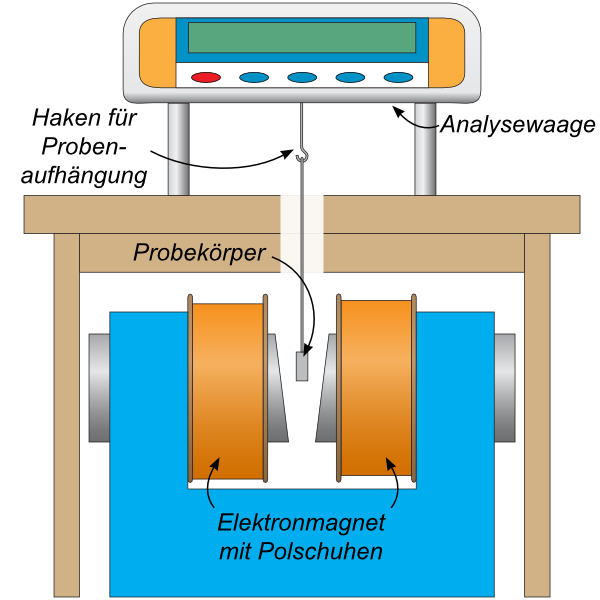
\includegraphics{aufbau}
	\caption{Aufbau der Waage zur Bestimmung der Kräfte.}
	\label{fig:aufbau}
\end{figure}
\begin{figure}[h]
	\centering
	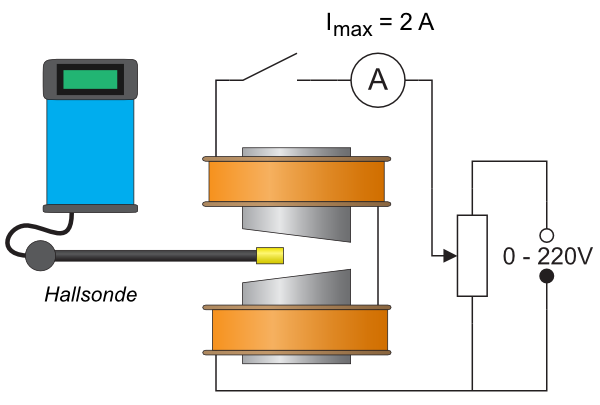
\includegraphics{schaltkreis}
	\caption{Schaltkreis zur Bestimmung von Dia- und Paramagnetismus.}
	\label{fig:schaltkreis}
\end{figure}

\section{Auswertung}
\label{sec:auswertung}
\begin{figure}[h]
\centering
\adjustbox{width=0.8\linewidth}{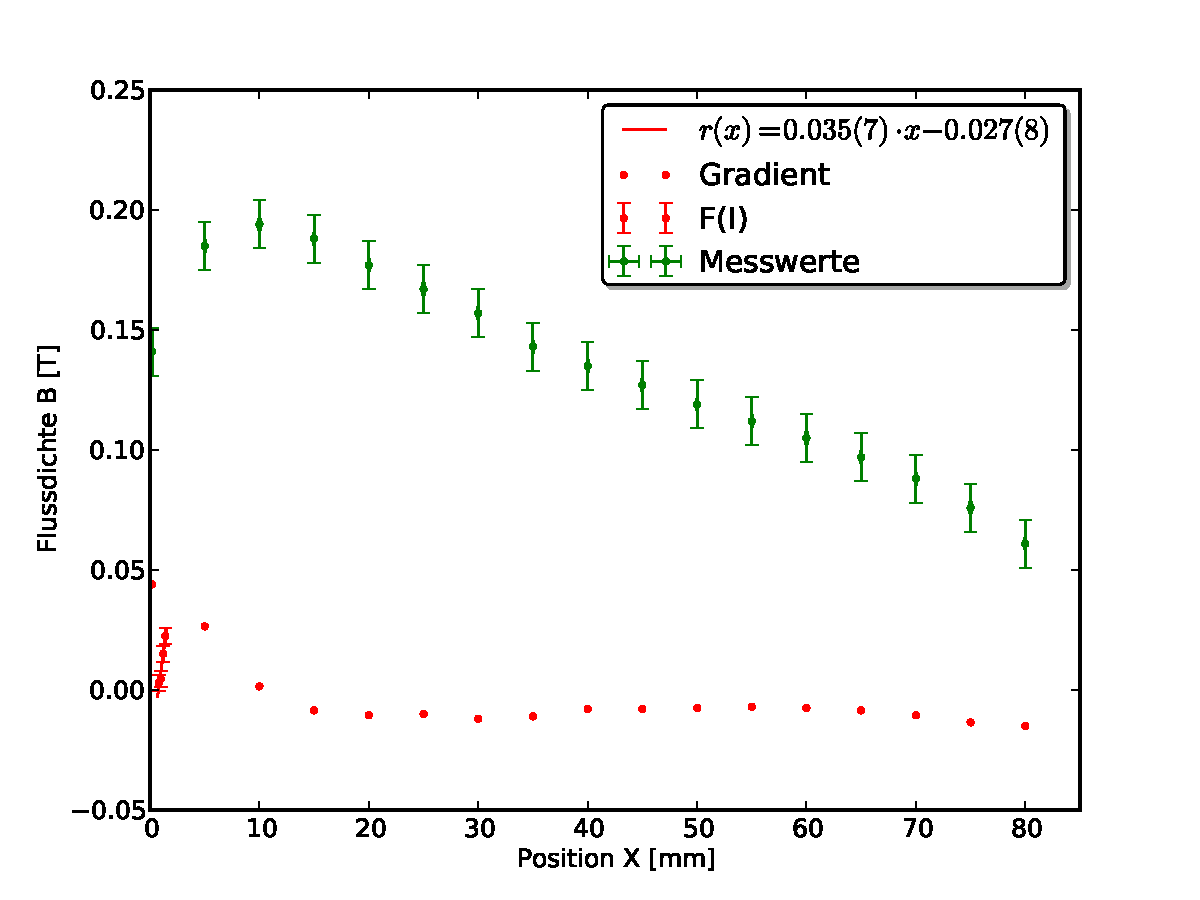
\includegraphics{Aus1}}
\caption{Auswertung von Versuch 1}
\label{fig:aus1}
\end{figure}
\begin{figure}[h]
\centering
\adjustbox{width=0.8\linewidth}{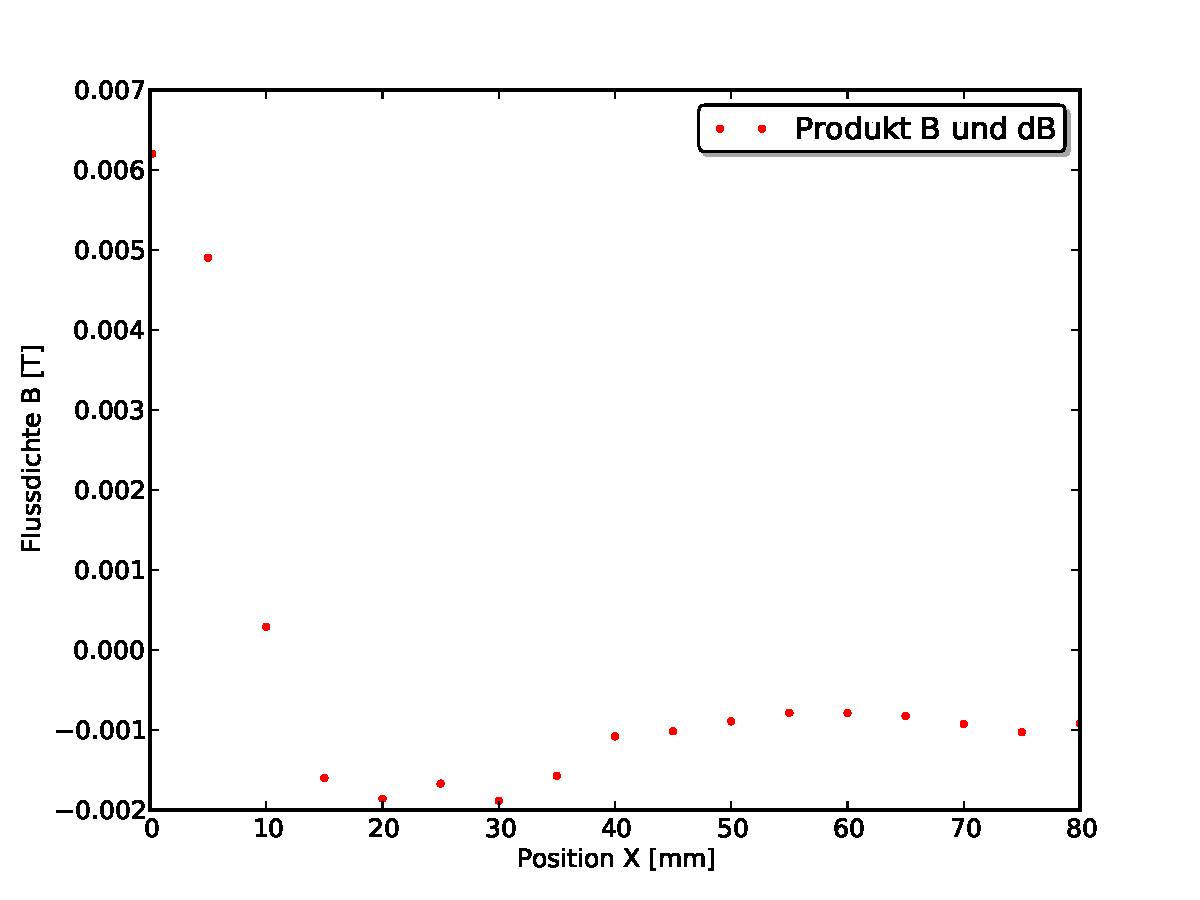
\includegraphics{Aus3}}
\caption{Auswertung von Versuch 3}
\label{fig:aus3}
\end{figure}
\begin{figure}[h]
\centering
\adjustbox{width=0.8\linewidth}{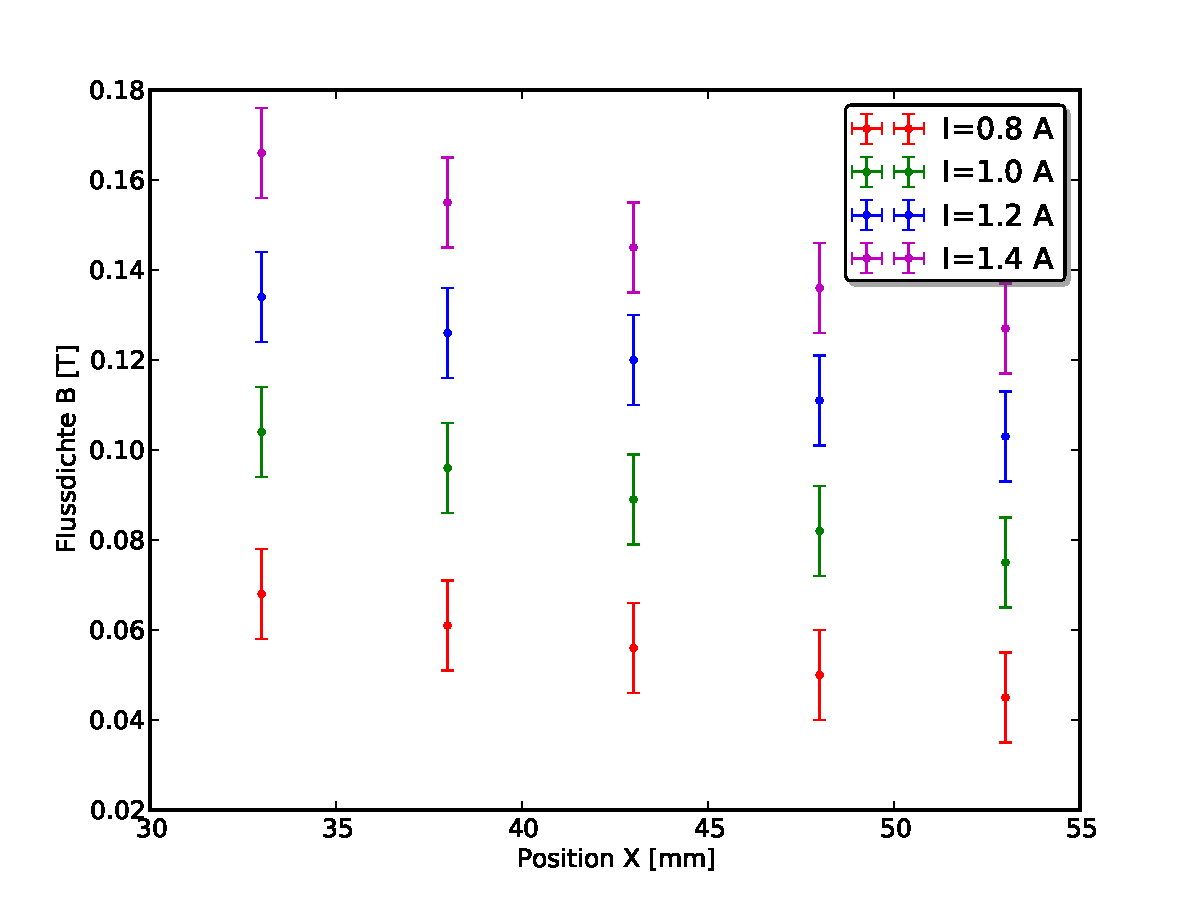
\includegraphics{Aus61}}
\caption{Auswertung von Versuch 6 erster Teil}
\label{fig:aus61}
\end{figure}
\begin{figure}[h]
\centering
\adjustbox{width=0.8\linewidth}{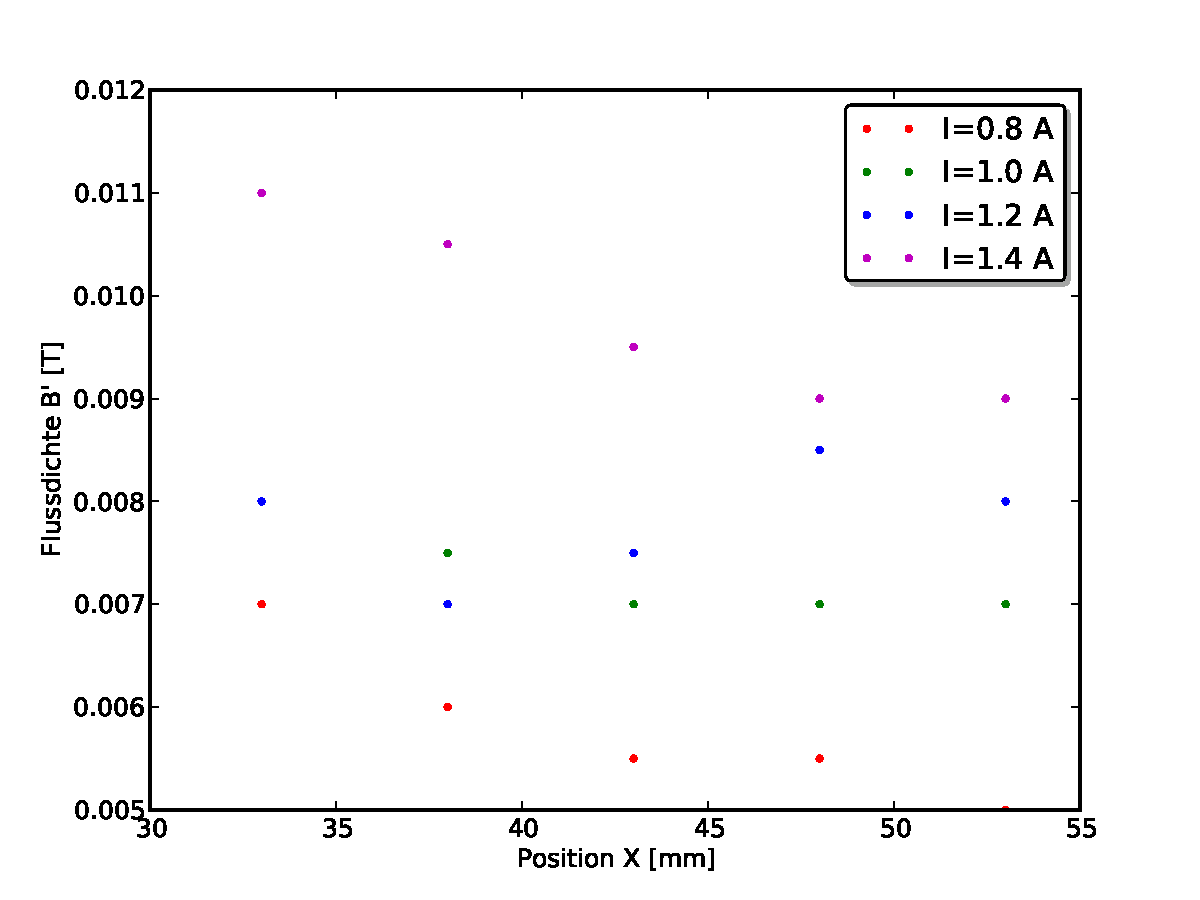
\includegraphics{Aus62}}
\caption{Auswertung von Versuch 6 zweiter Teil}
\label{fig:aus62}
\end{figure}
\begin{figure}[h]
\centering
\adjustbox{width=0.8\linewidth}{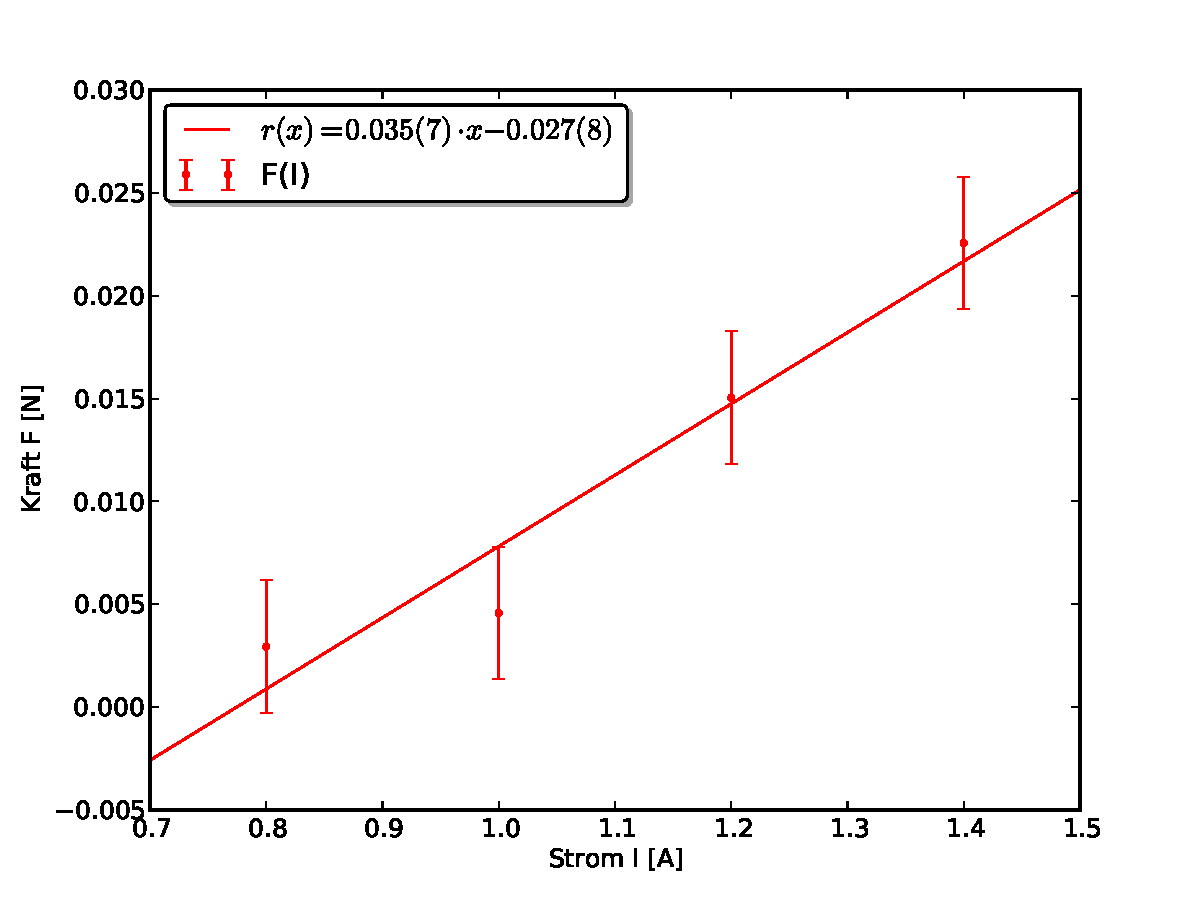
\includegraphics{Aus7}}
\caption{Auswertung von Versuch 7}
\label{fig:aus7}
\end{figure}

\section{Diskussion}
\label{sec:diskussion}

\bibliography{literatur}
\bibliographystyle{babalpha}
\end{document}
